\documentclass[10pt,a4paper]{report}
\usepackage[utf8]{inputenc}
\usepackage[english]{babel}
\usepackage[T1]{fontenc}
\usepackage{amsmath}
\usepackage{amsfonts}
\usepackage{graphicx}
\usepackage{lmodern}
\usepackage{amssymb}
\usepackage{verbatim}
\usepackage{float}
\usepackage{minitoc}
\usepackage{amsthm}
\newtheorem{definition}{Definição}
\newtheorem{theorem}{Teorema}
\usepackage{hyperref}
\title{\LARGE{Software Security} \\ \vspace{0.5cm} \normalsize{Summary}}
\date{}

\begin{document}
\maketitle
\tableofcontents

\chapter{Language Based Security}
\section{Information Flow Security}
\subsection{Tracking Information Flow}
Perl has a taint mode feature that allows the tracking of input. When active all forms of input to the programs are marked as "tainted". Tainted variables taint variables explicitly calculated from them and tainted data may not be used in any sensitive command (with some exceptions).\\
\\
This mechanism implicits a set of security classes (tainted vs. untainted), as well as a classification of objects/information holders, a specification of when information can flow from onde security class to another and a way to determine security classes that safely represent the combination of two other.
\subsection{Information Flow Policies}
The goals of information security are confidentiality and integrity. Information flow policies specify how information should be allowed to flow between objects of each security class. To define one such policy we need:
\begin{itemize}
\item A set of security classes
\item A can-flow relation between them
\item An operator for combining them
\end{itemize}
\subsubsection{Information Flow Policies For Confidentiality}
Confidentiality classes determine who has the right to read and information can only flow towards confidentiality classes that are at least as secret.\\
\\
Information that is derived from the combination of two security classes takes a confidentiality classes that are at least as secret as each of them.
\subsubsection{Information Flow Policies For Integrity}
Integrity classes determine who has the right to write and information can only flow towards integrity classes that are no more trustful.\\
\\
Information that is derived from the combination of two integrity classes takes an integrity class that is no more trustful than each of them.
\subsubsection{Formal Information Flow Policies}
These policies can be described as a triple $(SC, \rightarrow, \oplus)$, where:
\begin{itemize}
\item $SC$ is a set of security classes
\item $\rightarrow \subseteq SC \times SC$ is a binary can-flow relation on $SC$
\item $\oplus: SC \times SC \rightarrow SC$ is an associative and commutative binary class-combining or join operator on $SC$
\end{itemize}
Example high-low policy for confidentiality:
\begin{itemize}
\item $SC = \{H,L\}$
\item $\rightarrow = \{(H,H), (L,L), (L,H)\}$
\item $H \oplus H = H, L \oplus H = H, L \oplus L = L$
\end{itemize}
And for integrity:
\begin{itemize}
\item $SC = \{H,L\}$
\item $\rightarrow = \{(H,H), (L,L), (H,L)\}$
\item $H \oplus H = H, L \oplus H = L, L \oplus L = L$
\end{itemize}
\subsubsection{Partial Order Policies}
It often makes sense to assume that information can always flow within the same security level, security levels that are related to others in the same way are the same security level and, if information can flow from $A$ to $B$ and from $B$ to $C$, it can flow from $A$ to $C$. The flow relation $\rightarrow \subseteq SC \times SC$ is a partial order $(SC,\rightarrow)$ if it is:
\begin{itemize}
\item Reflexive: $\forall s \in SC, s \rightarrow s$
\item Anti-symmetric: $s_1 \rightarrow s_2$ and $s_2 \rightarrow s_1$ implies $s_1 = s_2$
\item Transitive: $s_1 \rightarrow s_2$ and $s_2 \rightarrow s_3$ implies $s_1 \rightarrow s_3$
\end{itemize}
When dealing with a partial order, the notation for $\rightarrow$ is $\leq$ and we can speak of security levels.\\
\\
Hasse diagrams are convenient for representing information flow policies that are partial orders. They are directed graphs where security classes are nodes, the can-flow relation is represented by non-directed arrows, implicitly directed upward and reflexive/transitive edges are implicit.
\subsection{Access Control to Information Flow Control}
Information flow control focuses on how information is allowed to flow once an access control is granted. Access control is the control of interaction between subjects and objects, by validating access rights of subjects to resources of the system.
\subsubsection{Discretionary Access Control (DAC)}
Restricts access based on the identity of subjects and a set of access permissions that can be determined by subjects.\\
\\
It has a limitation where access permissions might allow programs to, in effect, circumvent the policies. This can be done legally by means of information flows that are encoded in the program, or illegally, when vulnerabilities in programs and language implementations can be exploited by attackers.
\subsubsection{Mandatory Access Control (MAC)}
Restricts access based on security levels of subjects (their clearances) and objects (their sensitivity). Controls how information flows in a system based on whom is performing each access. It has limitations of restrictiveness and covert channels.
\subsection{Encoding and Exploiting Information Flows}
Objects may be classified as follows:
\begin{itemize}
\item Object - resource holding or transmitting information
\item Security class/label - specifies who can access objects of that class
\item Security labelling - assigns security classes to objects (statically or dynamically)
\end{itemize}
We use a  standard imperative language where information containers are variables, where $X_L$ denotes that a variable $X$ has security level $L$. The information flow policy is as follows:
\begin{figure}[H]
\centering
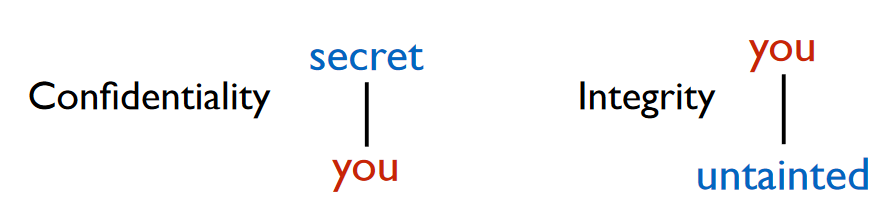
\includegraphics[scale=0.4]{1.png}
\end{figure}
We want to ensure that propagation of information by programs respects information flow policies, i.e. there are no illegal flows. This means an attacker cannot infer secret input or affect critical output by inserting inputs into the system and observing its outputs.

\chapter{Vulnerabilites And Secure Software Design}
In secure software design, there are 3 main security attributes: confidentiality, integrity and avaliability.
\section{Vulnerabilities}
A vulnerability is a system defect relevant security-wise, which may be exploited by an attacker to subvert security policy. Vulnerabilities may be classified as:
\begin{itemize}
\item Design vulnerabilities
\item Coding vulnerabilities
\item Operational vulnerabilities
\end{itemize}
\section{Attacks}
Attacks enter through interfaces, the attack surfaces. Attacks can be techincal or through social engineering, directed or not, manual or automated.
\subsection{Manual Attacks}
Some examples of manual attacks include:
\begin{itemize}
\item Footprinting
\item Scanning
\item Enumeration
\item Discovering vulnerabilites
\item ...
\end{itemize}
\subsection{Automated Attacks}
\subsubsection{Worm}
A worm is composed of a target selector, a scanning motor, a warhead (exploit code), a load and a propagation motor.
\subsubsection{Drive-by Download}
Performed by web pages with malware. When user accesses one with a vulnerable browser, the malware exploits the vulnerability.
\subsubsection{Viruses and Trojans}
Viruses are similar to worms but propagate with physical contact (usb drives, disks, ...). Trojans are also similar but requires the user to run an infected program (e.g. emails with attachments).
\subsection{Torpig}
Torpig is a sophisticated malware. It infects bots with drive-by download. Attackers modify legitimate but vulnerable server for some webpages to request JavaScript code from the attacker’s web server:
\begin{itemize}
\item[1] The victim’s browser accesses the vulnerable server
\item[2] JavaScript code exploits the browser/plugins/etc.
\item[3-4] If an exploit is successful, the script downloads and installs the Mebroot rootkit
(replaces Master Boot Record) – victim becomes a bot. Mebroot has no attack capacity.
\item[5] Contacts C\&C server to obtain malicious modules and stores them encrypted in directory system32 and changes the names and timestamps to avoid suspicions.\\
Every 2h contacts C\&C server: sends its configuration (type/version of modules); gets updates; communication is encrypted over HTTP
\item[6] Every 20 minutes contacts C\&C to upload stolen data
\item[7] When victim visits domain from a list (e.g., a bank), the bot contacts an injection server. Injection server returns attack data: URL of trigger page in the legitimate domain (typ. the login page), where to send results, etc.\\
When user visits trigger page, Torpig asks injection server for another page (e.g., that asks for credit card number)
\end{itemize}
\begin{figure}[H]
\centering
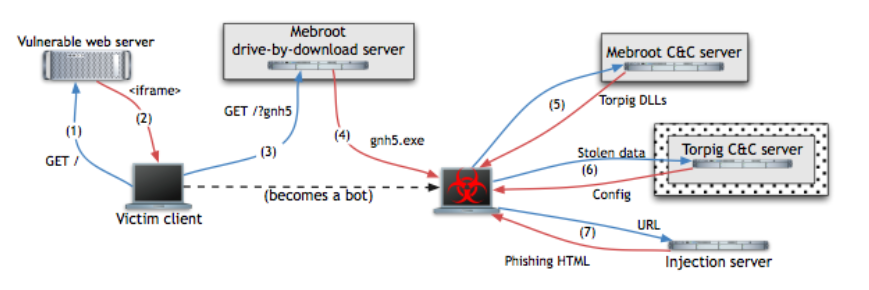
\includegraphics[scale=0.5]{2.png}
\end{figure}
\end{document}